% Optimization Project: Biscuit Optimizer
% Roberto Basla
% Politecnico di Milano
% A.Y. 2021/2022

\section{Modeling}
This section covers modeling approaches to the problem using AMPL, Google OR-Tools and Gurobi.

\subsection{Integer knapsack model}
The first approach consists in a relaxation of the problem that doesn't consider the placement of cutters on the dough: in this case only areas are considered, and the input image's mask $B$ is reduced to the number of available pixels (namely, $B = 13929$). Additional parameters are the cutter values $\underline{c}$ and cutter areas $\underline{a}$, while the integer vector $\underline{x}$ represents the number of times each cutter is selected (and is therefore the problem's variable).

This simpler problem consists in an integer knapsack that can be modeled as follows:
\begin{alignat}{3}
	\textrm{max}	&\quad& \sum_{i \in I}{c_i x_i}	& 				&& \label{eq:obj_knapsack} 		\\
	\textrm{s.t.}  	&\quad& \sum_{i \in I}{a_i x_i} & \leq B 		&& \label{eq:budget_knapsack} 	\\
					&\quad& x_i 					& \leq 3x_j		&& \quad \forall i \in I, \forall j \in I \label{eq:freq_knapsack} \\
					&\quad& x_i 					& \geq 0 		&& \quad \forall i \in I \label{eq:nonneg_knapsack} 
\end{alignat}

It maximizes the biscuit value multiplied by the number of times the cutter is used (\ref{eq:obj_knapsack}), subject to the knapsack's budget constraint (\ref{eq:budget_knapsack}) and the frequency constraints (\ref{eq:freq_knapsack}). Obviously, cutters must be selected a non-negative number of times (\ref{eq:nonneg_knapsack}).

As with any relaxation, the solution value is expected to be an upper bound for the complete problem.

\subsubsection{Results}
The model was solved very quickly by all three softwares, achieving a final value of $29000$ and a dough usage of 99.94\% of its pixels with the solution
$$
\underline{x} = 
\begin{bmatrix}
	4  \\
	4  \\
	4  \\
	11 \\
	4  \\
	12
\end{bmatrix}
$$

Figure \ref{fig:knapsack} shows the types of biscuits resulting from the optimization (39 in total). Models and results are available in the GitHub repository \href{https://github.com/rb-sl/biscuit_optimizer/tree/main/src/01-knapsack}{rb-sl/biscuit\_optimizer/src/01-knapsack}.

\begin{figure}[H]
	\centering	
	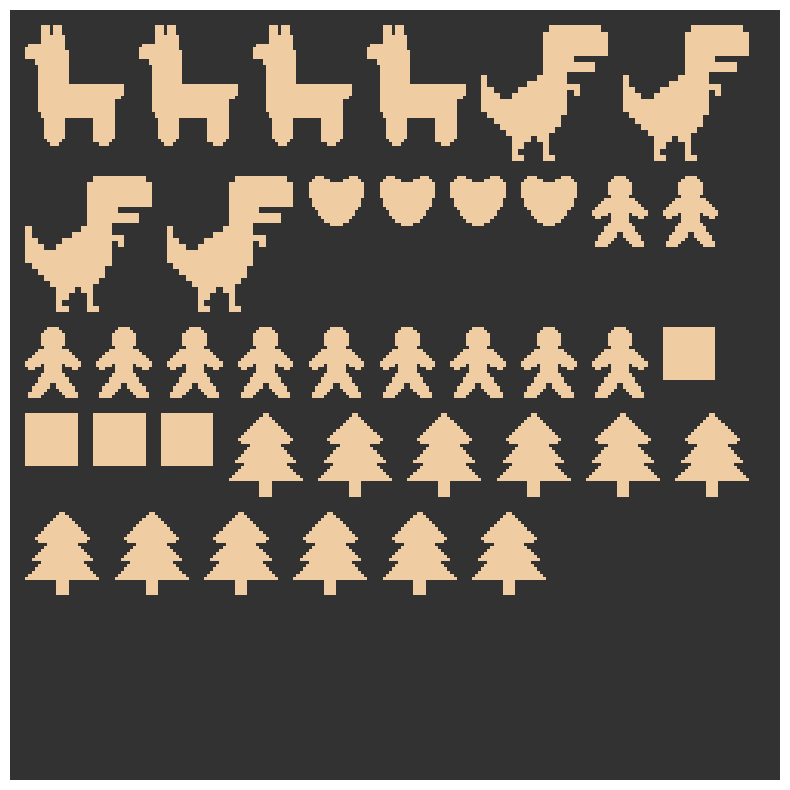
\includegraphics[width=.5\textwidth, keepaspectratio]{02-modeling/knapsack_visualization}
	\caption{Visualization of biscuits resulting from the knapsack problem}
	\label{fig:knapsack}
\end{figure}

\subsection{Nesting model}
The complete nesting model takes into account the initial mask and the cutter masks (so that they do not overlap). The solution is achieved through a set of binary variables $y$ over sets $I$ (the set of cutters), $N$ (the set of rows in the dough mask) and $M$ (the set of columns in the dough mask). $y_{i, n, m}$ is equal to 1 if a cutter $i$ is placed on the dough mask such that its top left corner is on the $(n, m)$ pixel in the mask.

In addition to sets and parameters already defined, the additional sets $\textrm{IN}_i$ and $\textrm{OUT}_i$ need to be defined as
\begin{alignat}{1}
	\textrm{IN}_i	& = \{(n, m): n \in N, m \in M, n + R_{i,max} \leq N_{max} \wedge m + C_{i,max} \leq M_{max} \} \notag \\
	\textrm{OUT}_i 	& = \{(n, m): n \in N, m \in M, n + R_{i,max} > N_{max} \vee m + C_{i,max} > M_{max} \} \notag
\end{alignat}
Naturally, it follows from the definition that $\textrm{IN}_i \cap \textrm{OUT}_i = \emptyset$ and $\textrm{IN}_i \cup \textrm{OUT}_i = B$, where $B$ represents the dough bitmask.
These sets need the additional parameters:
\begin{itemize}[itemsep=-1mm, topsep=-1mm]
	\item $N_{max}$: number of rows of the dough mask
	\item $M_{max}$: number of columns of the dough mask
	\item $R_{i,max}$: number of rows of cutter $i$
	\item $C_{i,max}$: number of columns of cutter $i$
\end{itemize}
Figure \ref{fig:in_out} shows an example of these sets and parameters for $i=1$.

\begin{figure}[H]
	\centering	
	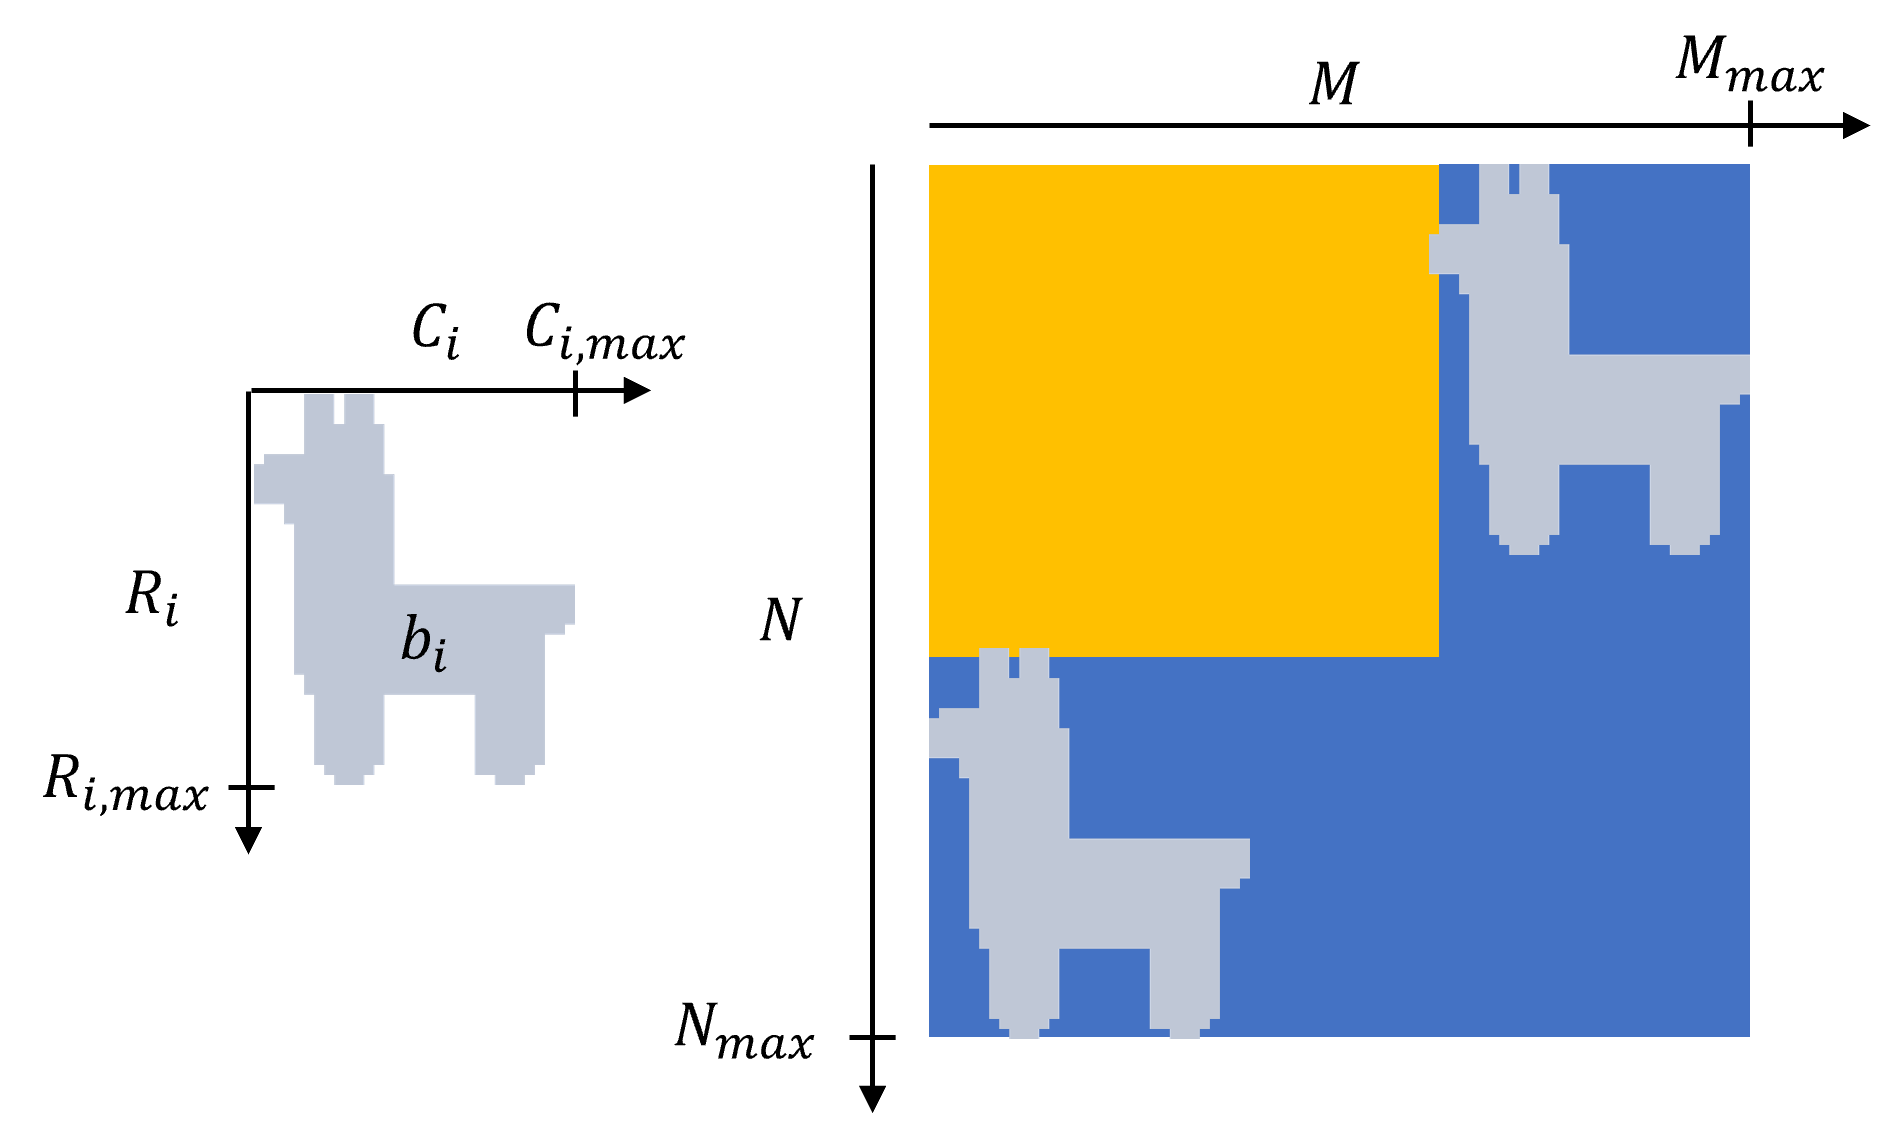
\includegraphics[width=.7\textwidth, keepaspectratio]{02-modeling/in_out}
	\caption{Examples of sets $\textrm{IN}_i$ (yellow) and $\textrm{OUT}_i$ (blue) for $i=1$}
	\label{fig:in_out}
\end{figure}

Finally, in order to help the formulation of the non-overlapping constraints, the integer variable $z$ is introduced over $I$, $N$ and $M$. $z_{i, n, m}$ represents the number of cutter masks $i$ that cover pixel $(n, m)$ (obviously, only the active part of a cutter mask influences $z$). Therefore, the complete nesting model is:
\begin{alignat}{3}
	\textrm{max}	& \sum_{i \in I}{c_i \sum_{n \in N}{\sum_{m \in M}{y_{i,n,m}}}} && \label{eq:obj_nest} \\
	\textrm{s.t.} \quad y_{i, n, m} & = 0 && \forall i \in I, \forall (n, m) \in \textrm{OUT}_i \label{eq:out_nest} \\
	y_{i, n, m} & \leq B_{n+h-1, m+k-1} + (1 - b_{i, h, k}) && \forall i \in I, \forall (n, m) \in \textrm{IN}_i, \notag \\
	& & & \forall h \in R_i, \forall k \in C_i \label{eq:in_nest} \\
	z_{i, n, m} & = \sum_{h \in R_i}{\sum_{k \in C_i}{y_{i,n-h+1, m-k+1}  b_{i, h, k}}} &\ & \forall i \in I, \forall n \in N, \forall m \in M \label{eq:link_nest} \\
	\sum_{i \in I}{z_{i, n, m}} & \leq 1 && \forall n \in N, \forall m \in M \label{eq:overlap_nest} \\
	\sum_{n \in N}{\sum_{m \in M}{y_{i,n,m}}} & \leq 3 \sum_{n \in N}{\sum_{m \in M}{y_{j,n,m}}} && \forall i \in I, \forall j \in I \label{eq:freq_nest} \\					
y_{i, n, m} & \in \{0, 1\} && \forall i \in I, \forall n \in N, \forall m \in M \label{eq:def_y} \\
z_{i, n, m} & \geq 0 && \forall i \in I, \forall n \in N, \forall m \in M \label{eq:def_z}
\end{alignat}

The objective function (\ref{eq:obj_nest}) is equivalent to the knapsack objective (\ref{eq:obj_knapsack}) (as $\sum_{n \in N}{\sum_{m \in M}{y_{i,n,m}}} = x_i \quad \forall i \in I$) and thus maximizes the overall value of chosen cutters. 

Constraint set (\ref{eq:out_nest}) enforces that the optimizer cannot place cutters that would result in partially cut-out biscuits due to the dough mask not being able to host them whole (thus operates on $\textrm{OUT}_i$); on the other hand, constraint set (\ref{eq:in_nest}) operates on the $\textrm{IN}_i$ sets and enforces that an $y_{i, n, m}$ may be selected only if the active pixels of cutter mask $i$ on $(n, m)$ fall on active pixels of the dough mask starting from $(n, m)$ up to $(n+R_i, m+C_i)$; it consists in the linearization of an AND operation. 

The set of linking constraints (\ref{eq:link_nest}) defines $z$ in function of $y$ so that the value of a $y_{i, n-h+1, m-k+1}$ (i.e., in the range defined by the cutter mask's dimension) is added to $z_{i, n, m}$ only if the cutter bitmask $b_{i, h, k}$ is active. Constraints (\ref{eq:overlap_nest}) enforce the non-overlapping property of the model by limiting the sum of active masks at each pixel $(n, m)$ in the dough mask.

Finally, constraints (\ref{eq:freq_nest}) enforce the maximum difference between the most frequently chosen cutter and the most infrequent. (\ref{eq:def_y}) and (\ref{eq:def_z}) define the variables.

\subsubsection{Results}
Due to the NP-Hard nature of the nesting problem, all solvers needed to be limited in time: the execution limit was set to 40000 seconds (some minutes less than 12 hours) for all instances. This decision may be the cause of the three optimizers finding different (locally optimal) solutions, unlike in the knapsack case where they were able to solve the problem exactly. It should be also noted that Python solutions added a small preprocessing, effectively merging constraints (\ref{eq:out_nest}) and (\ref{eq:in_nest}) in the form
\begin{lstlisting}[language=Python]
for i in I:
  for n in N:
    for m in M:
      if not can_host(dough_mask, cutter_mask, n, m):
        model.addConstr(y[n, m, i] == 0)
\end{lstlisting}
Effectively reducing the number of constraints by checking a priori with the \texttt{can\_host} function if a cutter $i$ could be placed in $(n, m)$ and, if not, just forcing $y_{i, n, m}$ to 0.

Models and results are available in the GitHub repository \\ \href{https://github.com/rb-sl/biscuit_optimizer/tree/main/src/02-nesting}{rb-sl/biscuit\_optimizer/src/02-nesting}.

\paragraph{AMPL solution}
The solution found by the CPLEX optimizer over the model defined in AMPL reached the objective of 16300 and is displayed in Figures \ref{fig:ampl_nest_overlay} and \ref{fig:ampl_nest_vis}.

\paragraph{OR-Tools solution} 
The CP-SAT optimizer solving the model defined in Google OR-Tools found a solution with value 17800, shown in Figures \ref{fig:ortools_nest_overlay} and \ref{fig:ortools_nest_vis}. Thanks to the possibility of adding callbacks every time a new solution is found, for this optimizer Figure \ref{fig:ortools_time} shows the plot of time against the best solution found. 

\paragraph{Gurobi solution}
Gurobi was able to reach the objective value of 17800 (using the same cutters) as well, but with a different configuration as shown in Figures \ref{fig:gurobi_nest_overlay} and \ref{fig:gurobi_nest_vis}.

\begin{figure}[H]
	\centering	
	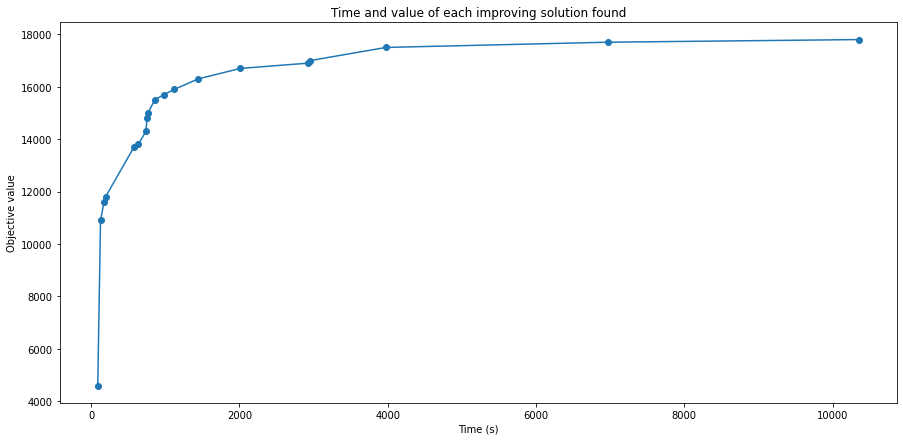
\includegraphics[width=\textwidth]{02-modeling/nest_ortools_time}
	\caption{Plot of the best current solution found by CP-SAT against time}
	\label{fig:ortools_time}
\end{figure}

\begin{figure}[p]
	\begin{subfigure}[b]{.43\textwidth}
		\centering
		\fbox{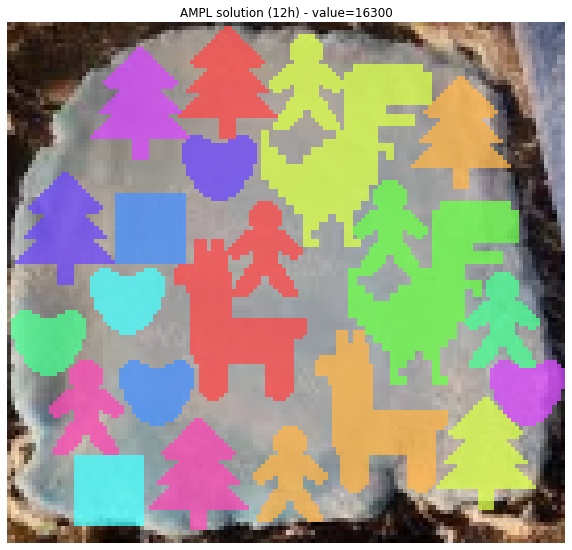
\includegraphics[width=\textwidth]{02-modeling/nest_ampl_overlay}}
		\caption{AMPL/CPLEX solution}
		\label{fig:ampl_nest_overlay}
	\end{subfigure} 
	\hfill
	\begin{subfigure}[b]{.43\textwidth}
		\centering
		\fbox{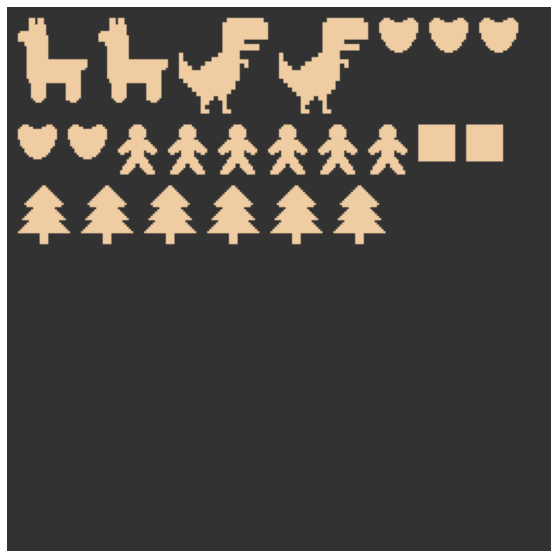
\includegraphics[width=\textwidth]{02-modeling/nest_ampl_visualization}}
		\caption{AMPL biscuits result}
		\label{fig:ampl_nest_vis}
	\end{subfigure}

	\vfill
	
	\begin{subfigure}[b]{.43\textwidth}
		\centering
		\fbox{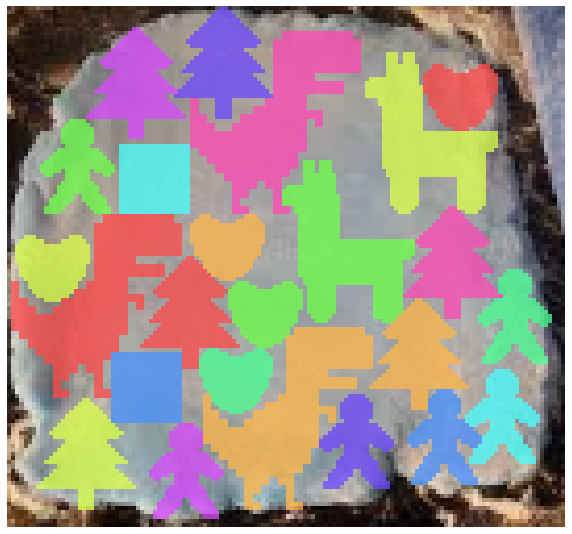
\includegraphics[width=\textwidth]{02-modeling/nest_ortools_overlay}}
		\caption{OR-Tools/CP-SAT solution}
		\label{fig:ortools_nest_overlay}
	\end{subfigure} 
	\hfill
	\begin{subfigure}[b]{.43\textwidth}
		\centering
		\fbox{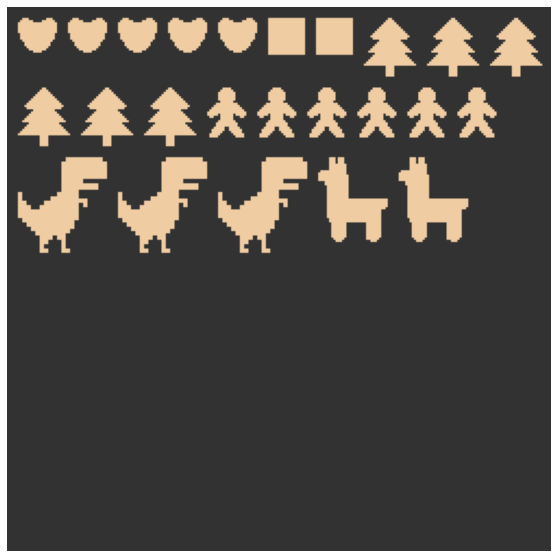
\includegraphics[width=\textwidth]{02-modeling/nest_ortools_visualization}}
		\caption{OR-Tools biscuits result}
		\label{fig:ortools_nest_vis}
	\end{subfigure}

	\vfill
	
	\begin{subfigure}[b]{.43\textwidth}
		\centering
		\fbox{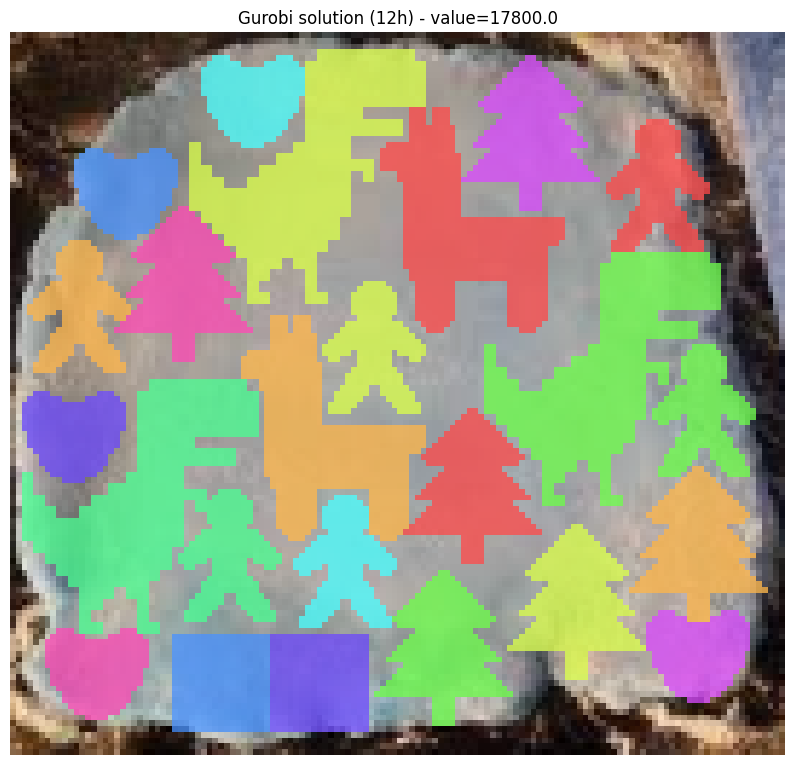
\includegraphics[width=\textwidth]{02-modeling/nest_gurobi_overlay}}
		\caption{Gurobi solution}
		\label{fig:gurobi_nest_overlay}
	\end{subfigure} 
	\hfill
	\begin{subfigure}[b]{.43\textwidth}
		\centering
		\fbox{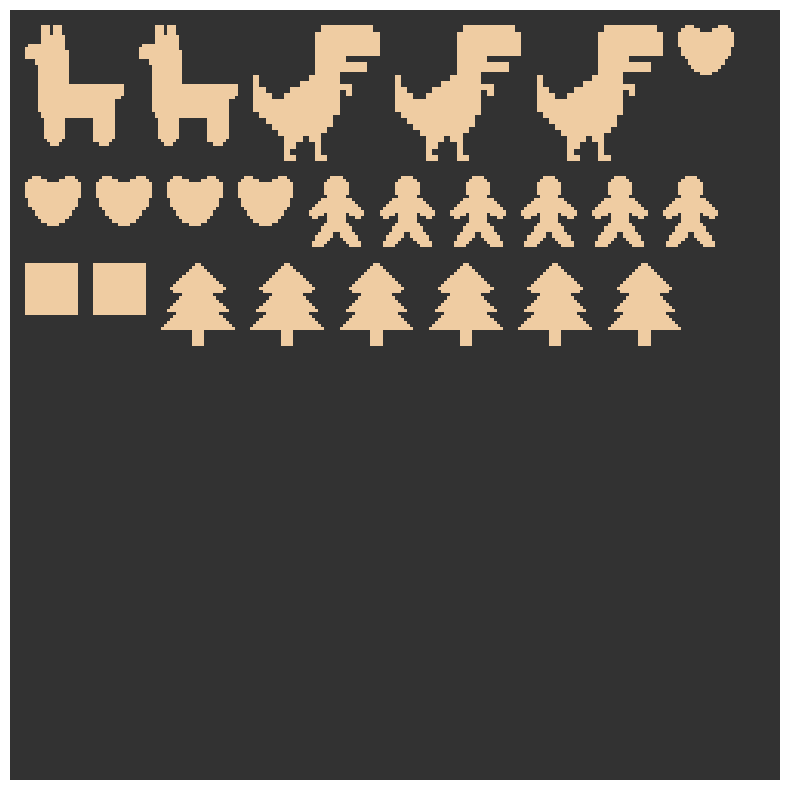
\includegraphics[width=\textwidth]{02-modeling/nest_gurobi_visualization}}
		\caption{Gurobi biscuits result}
		\label{fig:gurobi_nest_vis}
	\end{subfigure}
	\caption{Nesting results}
	\label{fig:nesting_results}
\end{figure}
